\subsection{Queue}
The queue will handle keeping track of requests made and their responses in the order that they are made

\begin{figure}[h!]
	\centering
 	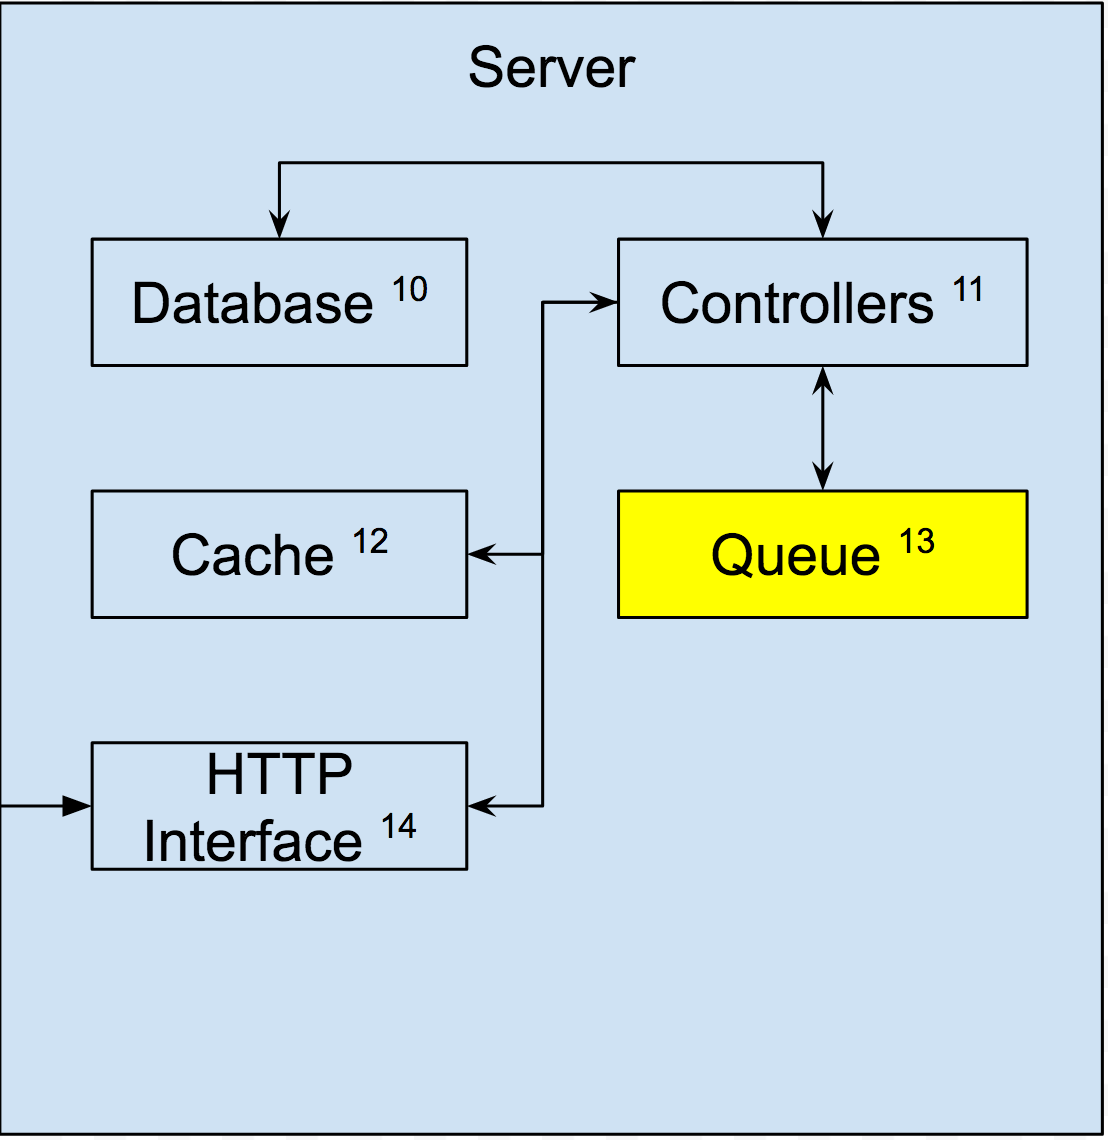
\includegraphics[width=0.60\textwidth]{images/server/server_queue.png}
 	\caption{Queue subsystem}
\end{figure}

\subsubsection{Assumptions}
N/A

\subsubsection{Responsibilities}
Making sure the requests/responses are kept in the correct order

\subsubsection{Subsystem Interfaces}
\begin {table}[H]
\caption {Queue interfaces} 
\begin{center}
    \begin{tabular}{ | p{1cm} | p{6cm} | p{2cm} | p{6cm} |}
    \hline
    ID & Description & Inputs & Outputs \\ \hline
    \#01 & Request is made from two different tabs & \pbox{2cm}{Songs} & \pbox{6cm}{Songs info returned in order of request made}  \\ \hline
    \end{tabular}
\end{center}
\end{table}

\newpage
